% !TeX spellcheck = en_GB
\chapter{Resource Management} % Load balancing
%Below should
%Having redundant systems provides a number of favourable traits like scalability and availability.

Resource management is a key activity in a distributed decentralised system.
A decentralised system consists of a number of nodes with various resources available. 
The primary resources important to the Siemens case are: Memory, Processing time, Network bandwidth and Hard drive I/O operations. %TODO review at intet mangler

Resource management should be fair, this means the nodes should have the workload distributed as evenly as possible.
There are different ways to handle this, some systems are able to split a single task up in equally large chunks for each node, in the Siemens case this is similar to the control algorithm that every turbine controller will need to run.
In a system where the tasks can be split evenly among the nodes, resource management logic might not be need as the system achieves a fair distribution by design, needless to say this can result in a much simpler design because of fewer components while avoid overhead due to resource management control algorithms. %and data aggregation functionality?
Others have many different tasks that can run independently of each other in the Siemens case this will be handling requests from users and secondary systems running outside the wind farm.
In the Siemens case the system currently is designed to at peak to handle a hundred simultaneously connected clients from outside the wind farm. This workload needs to distributed fairly when building a decentralised system therefore dedicated resource management logic is needed.

\section{Load Balancing}
Software responsible for handling resource management is often refereed to as a load balancer.
Load balancers come in different complexity and with the ability to manage resource in various ways.
From naively assigning clients with a round robin based algorithm to distributing connections based on resource monitoring.
Some Load balancers require client and or server integration some function completely independently.
The Siemens case uses standard protocol where the client application is build by a third party,
therefore client integration is not possible with all public interfaces, and is not investigated further.

The Siemens case needs a Load balancer system with the following properties:
\begin{itemize}
	\item Allow the decentralised system to behave like a single server for the clients
	\item Provides a single entry points for clients to connect to
	\item Monitors current available resources
	\item Support fail over
	\item Have minimum resource impact on the host machine
\end{itemize}

% % % DNS load balancers are not relevant to the Simens case. % % % %
%Different load balancing methods will are here briefly described:
%%Load balancing for large systems can be split in tiers.
%\paragraph{Dynamic DNS}
%is a load balancer built into the DNS service, it distributes load in a round robin manner as well as using region knowledge of where the request was revived from \cite{Amazon:Route53}. DNS based load balancing is among the most scalable solutions that does not need any special configuration of either client nor server. However is does not provide any monitoring of server performance parameters, and once the DNS lookup is over the service does not play any role in load balancing related to one that specific client until the DNS cache is refreshed. This type of loadbalancing is not applicable since 

A candidate for this kind of monitoring is the Linux Virtual Server project \cite{zhang2000linuxVirtualServer}.
At a lower tier it could be machine level based on performance parameters like , and finally application level based on the content of the request \textbf{[?]}. %\cite{Citation is missing and I need to find it}.
There exists a lot of solution specific load balancers.
A node balancer is a service witch distributes incoming requests, among the services registered on the network.
The distribution is based on different policies like dividing packages or picking the one with most free CPU capacity.
The load balancer could be a single point of failure, it should for this reason always have one or more backups as seen in \cref{fig:loadBalancingSetup}.
The load balancer monitors the real servers and only parses on requests to running servers.
A secondary needs to monitor the primary load balancer and step in if it stops responding.
This can be done using a virtual private IP, which is the address for all incoming requests. Also there exists solutions witch does all this in a completely distributed manner avoiding having a central server as load balancer  \textbf{[?]}, %\cite{Some cite I ahven't found yet}, 
this is even in some cases extended to include the clients in the act of load balancing \textbf{[?]}. % \cite{Some cite to netflix eureka balancer}.

\begin{figure}
	\centering	
	\scalebox{0.7}{\begin{tikzpicture}[
	start chain=going right,
	diagram item/.style={
		minimum width=80pt,
%		minimum height=45pt,
		on chain,
		join
	},
	diagram item seperated/.style={
			minimum width=80pt,
	%		minimum height=45pt,
			on chain
		}
]
\node [
	diagram item,
  label=center:Internet
] (Internet) {
\includegraphics{Cisco_BW/cloud}};

%\node [
%	continue chain=going below,
%	diagram item,
%	label=right:Router
%] {
\includegraphics{Cisco_BW/router}};

\node [
	start branch=1 going below right,
	diagram item seperated,
	label={[align=center]right:Load\\Balancer\\(Secondary)}
] (LB2) {
\includegraphics{Cisco_BW/distributed_director}};

\node [
	continue chain=going below left,
	diagram item,
	label={[align=center]left:Load\\Balancer\\(Primary)}
] (LB1) {
\includegraphics{Cisco_BW/distributed_director}};

\node [
	continue chain = going below right,
	diagram item,
	label={[align=center]right:Services in distrinbuted\\across the wind farm}
] (farm) {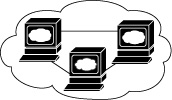
\includegraphics{Cisco_BW/web_cluster}};

\draw[loosely dotted] (LB1) -> (LB2) node[fill=white,midway]{heatbeat};
\draw[dashed] (Internet) -> (LB2);
\draw[dashed] (LB2) -> (farm);

\node [
	start branch=1 going below right,
	diagram item,
	label=below:Other interface
] {\includegraphics{Cisco_BW/PC}};

\node [
	start branch=1 going below left,
	diagram item,
	label=below:Http interface
] {\includegraphics{Cisco_BW/PC}};

\node [
	continue chain = going below,
	diagram item,
	label=below:Modbus interface
] {\includegraphics{Cisco_BW/PC}};

\end{tikzpicture}}
	\captionsetup{format=plain,font=footnotesize,labelfont={bf,defaultCapFont},labelsep=quad,singlelinecheck=no}
	\caption[Distributed System with 2 load balancing nodes]{
		\label{fig:loadBalancingSetup2Balancers} 
		\footnotesize{%
			A Distributed System with 2 load balancing nodes.
		}
	}
\end{figure}

In this solution the load balancer needs to balance external connections to different protocols like HTTP and Modbus, however a solution witch can be extended to any restful protocol is needed.
Also balancing of node roles depending on the amount incoming traffic on different interfaces will be needed.
Should all this be done automatically or is it better to define this manually???

Load balances can provide various features, related to offloading the real server and node management. % SSL decryprtion, caching, authentication, ...

 
\paragraph{consider the} 
\begin{itemize}
\item job migration cost
\item resource heterogeneity
\item network heterogeneity

\item traffic
\item resource usage
\item error
\item conditions
\end{itemize}

\paragraph{performance parameters}
\begin{itemize}
\item job size
\item data transfer rate
\item status exchange period
\item migration limit
\end{itemize}

\paragraph{Algorithms/policies}
\begin{itemize}
	%(On the Design of Adaptive and Decentralized	Load-Balancing Algorithms with Load Estimation for Computational Grid Environments)	
	\item MELISA Modified ELISA (used for large scale system (interGrid))
	\item LBA Load Balancing on Arrival
	
	\item Round-robin (Weighted/unweighed)
	\item Least-Connection (Weighted/unweighed)
\end{itemize}

\paragraph{The following requirements to the system exists}
\begin{itemize}
	\item Robustness
	\item Protocol flexible
	\item Must be a distributed component
\end{itemize}

\paragraph{Preferred features}
\begin{itemize}
	\item support TCP Handoffs (for non restful applications)
\end{itemize}

\section{Levels of balancing}
\begin{description}
	\item[??] DDNS / Round robin DNS
	\item[OSI 3] Network/IP %google says network layer LVS says transport layer
	\item[OSI 4] Network/IP
	\item[OSI 7] {Application level, like http balancing, allows balancing strategies based on url and user location.}
\end{description}

What we would like is a transport layer protocol.
\vspace{1cm}

\noindent\cite{Ludwig:SwarmIntelligenceGridLoadBalancing} 
Implements a particle swam based and an ant based algorithm. 
It discuses quality parameters.
It compares with a version using distributed knowledge (SBA State Broadcast Algorithm)
\\

\noindent\cite{MayuriMehta:HybridDynamicLB} Central and distributed Balancing (hybrid). Central(3) dosn't scale, distributed (6 refs) has a larger overhead. Implements node selection algorithms.



\section{Existing solutions}
\begin{description}
	\item [Linux Virtual Server: IPVS] Is implemented in the linux kernal version 2.4 and 2.6. Works at the IP level. Used by big sites sourceforge.net, layer 3.
	\item [Google Compute Engine: Load Balancer]: Proprietary. layer 3 and 7.
	%http://aws.amazon.com/route53/
	\item [Amazon Route 53] DNS based server, provides region based balancing and latency balancing.
	\item [AWS ELB] Amazons load balancer, Proxy based, top tier
	%https://github.com/Netflix/eureka/wiki/Eureka-at-a-glance
	\item [Eureka] Netflix Load Balancer, client based, middle tier
\end{description}

\begin{itemize}
	\item batch schedulers
	\item workflow engines
	\item operating systems (build in scheduler)
\end{itemize}

\begin{figure}
	\centering	
	\scalebox{0.7}{\begin{tikzpicture}[
start chain=going right,
diagram item/.style={
	minimum width=80pt,
	on chain,
	join
},
diagram item seperated/.style={
	minimum width=90pt,
	on chain
}]

\node [
diagram item,
label=above:Client 1
] (client1) {\includegraphics{Cisco_BW/PC}};

\node [
start branch=1 going right,
diagram item seperated,
label=above:Client 2
] (client2){\includegraphics{Cisco_BW/PC}};

\node [
continue branch=1 going right,
diagram item seperated,
label=above:Client 3
] (client3) {\includegraphics{Cisco_BW/PC}};

\node [
continue chain=going below right,
diagram item,
label=center:Internet
] (Internet) {
\includegraphics{Cisco_BW/cloud}};

\node [
start branch=1 going below right,
diagram item seperated,
label={[align=center]right:Load\\Balancer\\(Secondary)}
] (LB2) {
\includegraphics{Cisco_BW/distributed_director}};

\node [
continue chain=going below left,
diagram item,
label={[align=center]left:Load\\Balancer\\(Primary)}
] (LB1) {
\includegraphics{Cisco_BW/distributed_director}};

\node [
continue chain = going below right,
diagram item
] (farm) {};

\node [
start branch=1 going below right,
diagram item,
label=below:Client 3 Handler
] {\includegraphics{Cisco_BW/PC}};

\node [
start branch=1 going below left,
diagram item,
label=below:Client 1 Handler
] {\includegraphics{Cisco_BW/PC}};

\node [
continue chain = going below,
diagram item,
label=below:Client 2 Handler
] {\includegraphics{Cisco_BW/PC}};

%Lines to/from LB2
\draw[loosely dotted] (LB1) -> (LB2) node[fill=white,midway]{heatbeat};
\draw[dashed] (Internet) -> (LB2);
\draw[dashed] (LB2) -> (farm);

\draw (Internet) -> (client2);
\draw (Internet) -> (client3);


\end{tikzpicture}
}
	\captionsetup{format=plain,font=footnotesize,labelfont={bf,defaultCapFont},labelsep=quad,singlelinecheck=no}
	\caption[Routing requests as load balancing]{
		\label{fig:RoutingloadBalancingSetup} 
		\footnotesize{%
			Routing requests as load balancing.
		}
	}
\end{figure}

\begin{figure}
	\centering	
	\scalebox{0.7}{\begin{tikzpicture}[
start chain=going right,
diagram item/.style={
	minimum width=30pt,
	on chain
%	join
},
connection/.style={
%	->,
	thick,
	shorten <=2pt,
	shorten >=2pt,
}]

\newcounter{TurbnieCounter}

\newcommand\millFigure{
\includegraphics[width=0.5cm]{MillSiluet}}


\newcommand{\printTurbineID}{\ifnum\value{TurbnieCounter}<10 0\fi\arabic{TurbnieCounter}}
\stepcounter{TurbnieCounter}

\node [
diagram item,
label={[align=center]above:T\printTurbineID\\Load Balancer Active}
] (CenterNode) {\millFigure};
\stepcounter{TurbnieCounter}

\node [
draw,
below =2cm of CenterNode,
inner sep=0.5cm
%label={[align=center]left:T\printTurbineID\\LoadBalancer\\Primary}
] (Switch) {switch};
\draw[connection] (Switch) -- (CenterNode);


\node [
continue chain = going right,
diagram item,
label={[align=center]above:T\printTurbineID\\Spare}
] (Turbine) {\millFigure};
\stepcounter{TurbnieCounter}
\draw[connection] (Switch) -- (Turbine);

\node [
continue chain = going right,
diagram item,
label={[align=center]right:T\printTurbineID\\Spare}
] (Turbine) {\millFigure};
\stepcounter{TurbnieCounter}
\draw[connection] (Switch) -- (Turbine);

\node [
continue chain = going below,
diagram item,
label={[align=center]right:T\printTurbineID\\Spare}
] (Turbine) {\millFigure};
\stepcounter{TurbnieCounter}
\draw[connection] (Switch) -- (Turbine);

\node [
continue chain = going below,
diagram item,
label={[align=center]right:T\printTurbineID\\External\\Interface}
] (Turbine) {\millFigure};
\stepcounter{TurbnieCounter}
\draw[connection] (Switch) -- (Turbine);

\node [
continue chain = going below,
diagram item,
label={[align=center]right:T\printTurbineID\\Spare}
] (Turbine) {\millFigure};
\stepcounter{TurbnieCounter}
\draw[connection] (Switch) -- (Turbine);

\node [
continue chain = going left,
diagram item,
label={[align=center]below:T\printTurbineID\\Spare}
] (Turbine) {\millFigure};
\stepcounter{TurbnieCounter}
\draw[connection] (Switch) -- (Turbine);

\node [
continue chain = going left,
diagram item,
label={[align=center]below:T\printTurbineID\\Spare}
] (Turbine) {\millFigure};
\stepcounter{TurbnieCounter}
\draw[connection] (Switch) -- (Turbine);

\node [
continue chain = going left,
diagram item,
label={[align=center]below:T\printTurbineID\\Spare}
] (Turbine) {\millFigure};
\stepcounter{TurbnieCounter}
\draw[connection] (Switch) -- (Turbine);

\node [
continue chain = going left,
diagram item,
label={[align=center]left:T\printTurbineID\\Spare}
] (Turbine) {\millFigure};
\stepcounter{TurbnieCounter}
\draw[connection] (Switch) -- (Turbine);

\node [
continue chain = going above,
diagram item,
label={[align=center]left:T\printTurbineID\\Spare}
] (Turbine) {\millFigure};
\stepcounter{TurbnieCounter}
\draw[connection] (Switch) -- (Turbine);

\node [
continue chain = going above,
diagram item,
label={[align=center]left:T\printTurbineID\\Sparey}
] (Turbine) {\millFigure};
\stepcounter{TurbnieCounter}
\draw[connection] (Switch) -- (Turbine);

\node [
continue chain = going above,
diagram item,
label={[align=center]left:T\printTurbineID\\Spare}
] (Turbine) {\millFigure};
\stepcounter{TurbnieCounter}
\draw[connection] (Switch) -- (Turbine);

\node [
continue chain = going right,
diagram item,
label={[align=center]above:T\printTurbineID\\Spare}
] (Turbine) {\millFigure};
\stepcounter{TurbnieCounter}
\draw[connection] (Switch) -- (Turbine);



%\node [
%continue chain = going below,
%diagram item,	
%label={[align=center]right:T04\\LoadBalancer\\Primary}
%] (end1) {\millFigure};

%\draw (endBranch1) -> (end1) node{};
%\draw (endBranch1) -> (startBranch) node{};
%\draw (endBranch1) -> (start) node{};
%\draw (end1) -> (startBranch) node{};



%\draw (endBranch2) -> (end2) node{};

\end{tikzpicture}}
	\captionsetup{format=plain,font=footnotesize,labelfont={bf,defaultCapFont},labelsep=quad,singlelinecheck=no}
	\caption[System overview from the load balancer viewpoint]{
		\label{fig:loadBalancingSetup} 
		\footnotesize{%
			A system overview from the load balancer viewpoint.
		}
	}
\end{figure}















